
\section{Risposta ai segnali canonici}
Ci si riferirà principalmente alla risposta al gradino e all'impulso, facendo
uso della funzione di trasferimento presentata nella sezione precedente.
Si esegue inizialmente un'analisi di tipo ``asintotico'', per $t\to \infty$,
successivamente per $t\to 0$. Questo tipo di risposta non richiede l'analisi
puntuale delle equazioni del sistema, è necessario analizzare alcune
caratteristiche della funzione di trasferimento.

La risposta all'impulso è per definizione l'antitrasformata della funzione di
trasferimento
$$
W(t) = \Lap^{-1} [W(s)]
$$
Sviluppati i fratti, la funzione avrà la seguente forma
$$
W(t) = \Lap^{-1}\left[\frac{R_0}{s} + \frac{R_1}{s^2} +\ldots +
\frac{R_{g-1}}{s^g} + \frac{p_1}{s-p_1} + \frac{p_2}{s-p_2} + \ldots \right]
$$
I primi fratti (fino a $R_{g-1}$) sono associati ai poli nell'origine, seguono
i fratti associati ai poli reali ($p_i$) o eventualmente complessi e coniugati.

Il valore di $g$ permette di capire il tipo di sistema e se positivo, il numero
di poli nell'origine.
L'antitrasformata del primo termine è un gradino, del secondo è una retta, poi
una parabola e così via.
Tutti questi segnali (eccetto il primo che resta costante) divergeranno per
$t\to \infty$.

Si analizzano gli altri poli, se ne esiste almeno uno con parte reale positiva,
si avrà un esponenziale divergente nell'antitrasformata, se invece sono tutti a
parte reale negativa la loro somma convergerà.
$$\left\{
\begin{aligned}
\exists p_i &: \Re(p_i) > 0 \Rightarrow \text{Divergono} \\
\forall p_i &: \Re(p_i) < 0 \Rightarrow \text{Convergono} \\
\forall p_i &: \Re(p_i) < 0 \text{ e qualcuno sull'asse } \Im\ (m_a=1)
\end{aligned}\right.
$$
Il terzo caso prevede la presenza di poli a parte reale negativa più
qualcuno sull'asse immaginario, a parte reale
nulla ma con molteplicità algebrica pari ad uno, in questo caso si ha una
permanenza dell'uscita. Se invece la molteplicità algebrica degli autovalori a
parte reale nulla è maggiore di uno il sistema diverge.

Un sistema è \textbf{asintoticamente stabile} se e soltanto se
$$
\lim_{t\to +\infty} W(t) = 0
$$
ciò è garantito solo se \textit{tutti} i poli hanno parte reale negativa.

\newpage
\subsection{Poli dominanti}
Sono i poli con parte reale massima, origine dei modi che perdurano per più
tempo.
Si ipotizza che il sistema sia asintoticamente stabile, tutti i poli sono
contenuti nel semipiano sinistro.

Si supponga che il polo dominante sia \textit{reale}, asintoticamente il
comportamento è simile ad un sistema del primo ordine. Dopo un tempo pari a tre
o quattro volte la costante di tempo del polo dominante è indifferente
considerare solo la funzione associata a quel polo o l'intera funzione di
trasferimento.
$$
W(s) = K_B \frac{\prod_i (1+s\tau_{zi})
\prod_i\left(1+\frac{2\zeta_{zi}}{\omega_{nzi}}s + \frac{s^2}{\omega_{nzi}^2}
\right)}{ \prod_i (1+s\tau_{pi})
\prod_i\left(1+\frac{2\zeta_{pi}}{\omega_{npi}}s + \frac{s^2}{\omega_{npi}^2}
\right)  }
$$
Il tipo $g$, in un sistema asintoticamente stabile, può essere negativo o al
più pari a zero. Per $t \to \infty, s\to 0$ la funzione di
trasferimento tende inizialmente a
$$W(s)=K_B\frac{1}{1+s\tau_{pj}}$$
con $\tau_{pj}$ la
costante di tempo dominante associata al polo $j$-esimo. La semplificazione va
eseguita nella forma di \textit{Bode} e va preservato il guadagno statico, non
è possibile eseguirla nella forma di \textit{Evans}.


Si supponga che i poli dominanti siano una coppia di poli complessi e coniugati.
In questo caso il termine residuo sarebbe
$$
W(s)=K_B \frac{1}{1+\frac{2\zeta_{pi}}{\omega_{npi}}s +
\frac{s^2}{\omega_{npi}^2}
}
$$

Si considereranno dunque due tipi di sistemi, sistemi del primo ordine o
sistemi del secondo ordine.
\newpage
\subsection{Sistema del primo ordine}
Sia il seguente sistema con funzione di trasferimento del primo ordine, si
studia la risposta all'impulso come antitrasformata della funzione di
trasferimento
$$
W(s) = K_B \frac{1}{1+s\tau} \stackrel{\Lap^{-1}}{\longrightarrow} W(t) = K_B
e^{-\frac{t}{\tau}}\cdot \delta_{-1}(t)
$$
\begin{figure}[h]
 \centering
 \begin{tikzpicture}
  \begin{axis}[
   width = 0.4\linewidth,
   axis lines = left,
   ylabel={$W(t)$},
   xlabel={$t$},
   xtick={0,1},
   xticklabels={,$\tau$},
   ytick={1},
   yticklabels={$K_B$},
   xlabel style={at={(ticklabel* cs:1)},anchor=north},
   ylabel style={at={(ticklabel* cs:1)},anchor= east,rotate=-90},
   ymax=1.3,
   ymin=0,
   ]
   \addplot[domain=0:3]{exp{-x}};
   \addplot[domain=0:1]{1-x};
\addplot [draw=none,pattern = north east lines, pattern color=red,
] coordinates {
    (0, 1.4)
    (0, 0)
    (0.5, 0)
    (0.5, 1.4)
};
  \end{axis}
 \end{tikzpicture}
\end{figure}
Questa soluzione vale per i sistemi del primo ordine e anche per quelli che si
approssimano per $t>\tau_{\text{max}}$ a sistemi del primo ordine, nel secondo
caso però le soluzioni per $t<\tau$ devono essere verificate rispetto alle
altre costanti di tempo del sistema.

\subsubsection{Risposta al gradino}
$$
u(t) = \delta_{-1}(t) \longrightarrow Y_f(s) = \frac{W(s)}{s} =
\frac{K_b}{s(1+s\tau)}
$$
antitrasformando si ottiene la risposta al gradino chiamata anche risposta
\textit{indiciale}.
$$\begin{aligned}
W_{-1}(t) &= \Lap{-1}
\left[\frac{K_B}{\tau}\left(\frac{R_0}{s}+\frac{R_1}{s+\frac{1}{\tau}}
\right)\right] = \Lap{-1}
\left[\frac{K_B}{\tau}\left(\frac{\tau}{s}+\frac{-\tau}{s+\frac{1}{\tau}}
\right)\right] = \\
&=K_B\left(1-e^{-\frac{t}{\tau}} \right)\delta_{-1}(t)
\end{aligned}$$
\begin{figure}[h]
 \centering
 \begin{tikzpicture}
  \begin{axis}[
   width = 0.4\linewidth,
   axis lines = left,
   ylabel={$W_{-1}(t)$},
   xlabel={$t$},
   xtick={0,1},
   xticklabels={,$\tau$},
   ytick={1},
   yticklabels={$K_B$},
   xlabel style={at={(ticklabel* cs:1)},anchor=north},
   ylabel style={at={(ticklabel* cs:1)},anchor= east,rotate=-90},
   ymax=1.3,
   ymin=0,
   ]
   \addplot[domain=0:3]{1-exp{-x}};
   \addplot[domain=0:1]{x};
   \addplot[dashed,domain=0:3]{1};
   \addplot[dashed]coordinates{(1,0) (1,1)};
\addplot [draw=none,pattern = north east lines, pattern color=red,
] coordinates {
    (0, 1.4)
    (0, 0)
    (0.5, 0)
    (0.5, 1.4)
};
  \end{axis}
 \end{tikzpicture}
\end{figure}
Anche in questo caso bisogna porre attenzione alle analisi condotte vicino lo
zero se il sistema del primo ordine è stato ottenuto come semplificazione di un
sistema  più complesso.

\subsection{Sistema del secondo ordine con poli complessi e coniugati}
La funzione di trasferimento ha la seguente forma
$$
W(s) = K_B \frac{1}{1+\frac{2\zeta}{\omega_n}s+\frac{s^2}{\omega_n^2}}
$$
\begin{figure}[h]
 \centering
 \begin{tikzpicture}
  \begin{axis}[
   width = 0.6\linewidth,
   axis lines = middle,
   axis equal image,
   ylabel={\Im},
   xlabel={\Re},
   ytick={-0.557,0.557},
   xtick={-0.706,0},
   xticklabels={$\alpha$,$0$},
   yticklabels={$-j\omega$,$j\omega$},
   y tick label style={anchor=west,xshift=0.5em},
   x tick label style={xshift=0.5em},
   xlabel style={at={(ticklabel* cs:1)},anchor=north west},
   ylabel style={at={(ticklabel* cs:1)},anchor= west,},
   xmax=1,
   xmin=-1,ymax=1,ymin=-1,
   ]
   \addplot[trig format plots=rad, domain=0:2*pi,samples=100]
   ({0.9*cos(x)},
    {0.9*sin(x)});

\draw[color=red] (0,0)--(-0.706,0.557) node[midway,above]{$\omega_n$};
\draw[color=red,->] (0,0.8) arc (90:141.73:0.8) node at (115.85:0.7){$\theta$};

    \draw[dashed] (0,-0.557) -- (-0.706,-0.557)node[circle,fill,
inner sep=2pt,]{} -- (-0.706,0.557)node[circle,fill,
inner sep=2pt]{} -- (0,0.557);
  \end{axis}
 \end{tikzpicture}
\end{figure}
L'angolo $\theta$ è tale che il coefficiente di smorzamento
$\zeta=\sin\theta$.\\
La pulsazione naturale $\omega_n$ è il modulo del polo dunque $\alpha = -
\omega_n\zeta$.

\subsubsection{Risposta all'impulso}
Si prova a calcolare la risposta all'impulso, riorganizzando la funzione di
trasferimento
$$
W(t) = \Lap^{-1}[W(s)] =
\Lap^{-1}\left[\frac{K_B}{\sqrt{1-\zeta^2}}\frac{\omega_n^2
\sqrt{1-\zeta^2}}{(s+\zeta\omega_n)^2+\omega_n^2(1-\zeta^2 ) } \right]
$$
Si esegue l'antitrasformata ottenendo una funzione seno.
$$
W(t) = \frac{K_B}{\sqrt{1-\zeta^2}}\omega_n e^{-\zeta\omega_n t}
\sin\left(\omega_n\sqrt{1-\zeta^2}\cdot t\right)\delta_{-1}(t)
$$
\newpage
Si ottiene un andamento identico a quanto analizzato alla sezione
\ref{sec:modo_pseudo_periodico}
\begin{figure}[h]
\centering
  \begin{tikzpicture}
   \begin{axis}[
     axis lines=left,
     axis x line=middle,
     width=0.6\textwidth,
     xtick={0,3},
     xticklabels={0,t},
     ytick={-1,0,1,1.5},
     xmax=3,
     ymax=1.5,
     ymin=-1,
     yticklabels={$-\frac{K_B}{\sqrt{1-\zeta^2}}\omega_n$,0,
$\frac{K_B}{\sqrt{1-\zeta^2}}\omega_n$,$W(t)$},
     ]
    \addplot[color=black,domain=0:3,samples=200]{exp(-x)*sin(500*x)};
    \addplot[color=red,domain=0:3]{exp(-x)}
         node[above,midway,color=red,yshift=1em]{$e^{-\zeta\omega_n t}$};
    \addplot[color=red,domain=0:3]{-exp(-x)}
         node[below,midway,color=red,yshift = -1em]{$-e^{-\zeta\omega_n t}$};
\addplot [draw=none,pattern = north east lines, pattern color=red,
] coordinates {
    (0, 1.6)
    (0, -1.1)
    (0.5, -1.1)
    (0.5, 1.6)
};
   \end{axis}
 \end{tikzpicture}
\end{figure}
Anche in questo caso se il sistema proviene da una semplificazione di un
sistema più complesso si devono trascurare le soluzioni ottenute per intervalli
di tempo troppo piccoli in funzione delle costanti di tempo eliminate.

\subsubsection{Risposta al gradino}
La funzione di uscita sarà pari a
$$
Y_f(s) = \frac{W(s)}{s} = K_B\frac{\omega_n^2}{s(\omega_n^2 + 2\zeta\omega_n s
+s^2)}
$$
antitrasformando
$$
W_{-1}(t) = K_B \Lap^{-1} \left[\frac{R_0}{s} + \frac{R_as+R_b}
{\omega_n^2 +2\zeta\omega_n s+s^2}\right]
$$
Con la formula dei residui $R_0=1$
$$
W_{-1}(t) = K_B \Lap^{-1} \left[\frac{(s^2+2\zeta\omega_n+\omega_n^2)
+R_as^2+R_bs}
{s(s^2+2\zeta\omega_n+\omega_n^2)}\right]
$$
Per il principio di identità dei polinomi i due numeratori devono essere
identici dunque mentre il coefficiente $\omega_n^2$ è già presente in entrambi
i termini, i coefficienti che moltiplicano $s$ ed $s^2$ devono annullarsi.
$$\left\{\begin{aligned}
&1+R_a = 0\\
&2\zeta\omega_n + R_b = 0
\end{aligned}\right.\longrightarrow
\begin{aligned}
R_a &= -1\\
R_b &= -2\zeta\omega_n
\end{aligned}
$$

Sostituendo i residui si riprende l'antitrasformata della risposta al gradino
$$\begin{aligned}
W_{-1}&(t) = K_B\Lap^{-1}\left[ \frac{1}{s}-\frac{s+2\zeta\omega_n}
{s^2+2\zeta\omega_ns+\omega_n^2} \right]=
K_B\Lap^{-1}\left[\frac{1}{s} - \frac{s+2\zeta\omega_n}
{(s+\zeta\omega_n)^2+\omega_n^2(1-\zeta^2)}
\right]=\\
&=K_B\Lap^{-1}\left[\frac{1}{s} -
\frac{s+\zeta\omega_n}{(s+\zeta\omega_n)^2
+\omega_n^2(1-\zeta^2)}- \frac{s}{\sqrt{1-\zeta^2}}
\frac{\omega_n\sqrt{1-\zeta^2}}{(s+\zeta\omega_n)^2 +
\omega_n^2(1-\zeta^2)}\right]=\\
&=K_B\left(1 -e^{-\zeta\omega_n t}\left(\cos\left(\omega_n\sqrt{1-\zeta^2}\cdot
t\right)+
\frac{\zeta}{\sqrt{1-\zeta^2}}
\sin\left(\omega_n \sqrt{1-\zeta^2}\cdot t\right)\right)
\right)\delta_{-1}(t)
\end{aligned}$$

Si ricorda una forma dell'identità trigonometrica
$$\begin{aligned}
&a\sin x + b\cos x = \sqrt{a^2+b^2}\sin\left(x+\varphi\right)\\
&\varphi = \arctan\left(\frac{b}{a}\right) =
\arccos\left(\frac{a}{\sqrt{a^2+b^2}}\right) =
\arcsin\left(\frac{b}{\sqrt{a^2+b^2}}\right)
\end{aligned}
$$
Applicandola alla precedente
$$
W_{-1}(t) = K_B\left( 1-\frac{1}{\sqrt{1-\zeta^2}}e^{-\zeta\omega_n
t}\sin\left( \omega_n\sqrt{1-\zeta^2}\cdot t + \arccos(\zeta) \right)
\right)\delta_{-1}(t)
$$

\begin{figure}[h]
\centering
  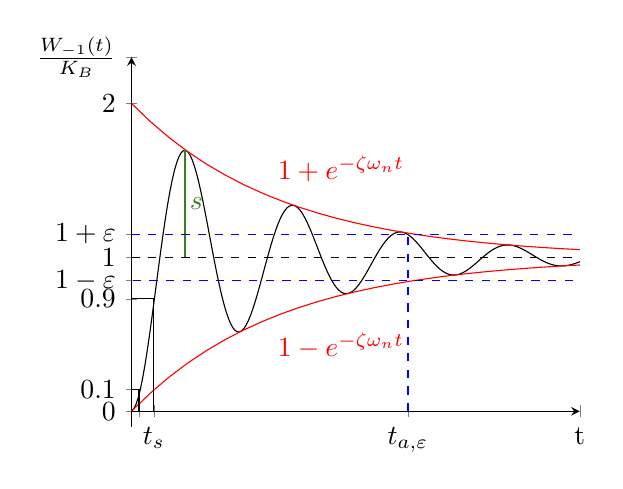
\begin{tikzpicture}
   \begin{axis}[
     axis lines=left,
     axis x line=middle,
     width=0.6\textwidth,
     xtick={0,0.05,0.15,1.85,3},
     xticklabels={0, ,$t_s$,$t_{a,\varepsilon}$,t},
     ytick={0,0.14,0.73,0.85,1,1.15,2,2.3},
     xmax=3,
     ymax=2.3,
     ymin=-0.1,
     yticklabels={0,0.1,0.9,$1-\varepsilon$,
1,$1+\varepsilon$,2,$\frac{W_{-1}(t)}{K_B}$},
     ]
    \addplot[color=black,domain=0:3,samples=200]{1-exp(-x)*sin(500*(x+1.61))};
    \addplot[color=red,domain=0:3]{1+exp(-x)}
         node[above,midway,color=red,yshift=1em]{$1+e^{-\zeta\omega_n t}$};
    \addplot[color=red,domain=0:3]{1-exp(-x)}
         node[below,midway,color=red,yshift = -1em]{$1-e^{-\zeta\omega_n t}$};
    \draw[dashed] (0,1)--(3,1);
% \addplot [draw=none,pattern = north east lines, pattern color=red,
% ] coordinates {
%     (0, 2.6)
%     (0, -1.1)
%     (0.2, -1.1)
%     (0.2, 2.6)
% };
\draw [color=OliveGreen,line width = 0.3mm] (0.36,1)--(0.36,1.7)
node[midway,xshift=0.4em]{$s$};
\draw [dashed,color = blue] (0,1.15)--(3.1,1.15)--(3.1,0.85)--(0,0.85);
\draw[dashed,color=blue](1.85,0)--(1.85,1.15);
\draw[](0,0.14)--(0.05,0.14)--(0.05,0);
\draw[](0,0.73)--(0.15,0.73)--(0.15,0);
   \end{axis}
 \end{tikzpicture}
\end{figure}
Si misura con $s$ il parametro detto \textit{sovraelongazione massima}, valore
percentuale che indica di quanto la funzione si ``sovraelonga'' ossia assume
valori maggiori di quello di regime $K_B$, aumenta al diminuire dello
smorzamento $\zeta$.

Si indica con $t_{a,\varepsilon}$ il tempo di assestamento, con $\varepsilon$
pari solitamente all'1\%, il 2\% o il 3\%. Si valuta da quale istante di tempo
in poi la funzione si confina nella banda di assestamento.

È facile dimostrare che il tempo di assestamento dipende dall'inviluppo
esponenziale
$$
t_{a,\varepsilon} = -\frac{1}{\zeta\omega_n}\ln(\varepsilon)
$$
con $\varepsilon$ espressa in percentuale.

Il tempo di \textit{salita} $t_s$ (o $t_r$ dall'inglese \textit{rise}) indica in
quanto tempo il segnale passa da un valore del 10\% ad un valore del 90\%
rispetto a quello di regime.

Si riporta l'andamento qualitativo della sovraelongazione $s$ in funzione di
$\zeta$.
\begin{figure}[h]
 \centering
 \begin{tikzpicture}
 \begin{axis}[
     axis lines=middle,
     width=0.6\textwidth,
     xlabel=$\zeta$,
     ylabel=$s$,
     xtick={0,0.1,0.2,0.6,1},
     ytick={0,0.1,0.5,0.7,1},
     xmax=1.2,
     xmin=-0.1,
     ymin=-0.1,
     ymax=1.2,
     ]
 \addplot[domain=0:1]{exp((-pi*x)/sqrt(1-x^2))};
 \draw[dashed](0,0.7)--(0.1,0.7)--(0.1,0);
 \draw[dashed](0,0.5)--(0.2,0.5)--(0.2,0);
 \draw[dashed](0,0.1)--(0.6,0.1)--(0.6,0);
 \end{axis}
 \end{tikzpicture}
\end{figure}
Sono riportati in figura alcuni valori convenzionali assunti dalla funzione.

\newpage
\subsection{Analisi con la forma di Evans}
Si analizzano i sistemi per $t\to 0^+$, si pone la funzione di trasferimento
nella forma di Evans con $K_E=\frac{b_m}{a_n}$
$$
W(s) = \frac{b_ms^m + \ldots + b_0}{a_ns^n + \ldots + a_0} =
K_E\frac{\prod_i(s-z_i)}{\prod_i (s-p_i)}
$$

Si calcola il limite della risposta all'impulso $W(t)$
mediante il teorema del valore iniziale.
$$
\lim_{t\to 0^+}W(t) = \lim_{s\to+\infty} sW(s)
$$
Per $s\to+\infty$ si considerano le potenze massime $s^n$ ed $s^m$ con
$n\geq m$ nei casi studiati
$$
\lim_{s\to+\infty} sW(s) = \left\{
\begin{aligned}
&K_E\delta(t) & &  \qquad n=m\\
&K_E\delta_{-1}(t) & &\qquad n-m=1\\
&0 & &\qquad n-m>1
\end{aligned}\right.
$$
Riassunto delle analisi per $t\to 0$.
\begin{table}[h]
\centering
\begin{tabular}{*{5}{c}}\toprule
\diagbox[width=6em]{$u(t)$}{$n-m$} & 0 & 1 & 2 & 3 \\ \midrule
$\delta(t)$ & $K_E\delta(t)$ & $K_E\delta_{-1}(t)$ & $K_E\delta_{-2}(t)$ &
$K_E\delta_{-3}(t)$ \\ \midrule
$\delta_{-1}(t)$ & $K_E\delta_{-1}(t)$ & $K_E\delta_{-2}(t)$ &
$K_E\delta_{-3}(t)$ & $K_E\delta_{-4}(t)$ \\ \midrule
$\delta_{-2}(t)$ & $K_E\delta_{-2}(t)$ & $K_E\delta_{-3}(t)$ &
$K_E\delta_{-4}(t)$ & $K_E\delta_{-5}(t)$\\ \bottomrule
\end{tabular}
\end{table}
Per studiare gli andamenti in sistemi di tipo 2 e 3 si studia la derivata
prima e seconda della risposta all'impulso
$$
\lim_{t\to0^+} \dot{W}(t) = \lim_{s\to +\infty} s^2W(s)=
\left\{\begin{aligned}
&K_E\delta_{-1}(t) & &  \qquad n-m=2\\
&0 & &\qquad n-m>2
\end{aligned}\right.
$$
Si vede che si ottengono le funzioni $\delta_{-n}$ ricavate
precedentemente nella sezione \ref{sec:segnali_canonici}.

Per la risposta al gradino si ottengono gli stessi casi ``traslati''
$$
\lim_{t\to 0^+} W_{-1}(t) = \lim_{s\to +\infty}
\cancel{s}\frac{W(s)}{\cancel{s}} = \left\{
\begin{aligned}
&K_E\delta_{-1}(t) & & \qquad n-m=0\\
&0 & & \qquad n-m>0
\end{aligned}\right.
$$
Si può iterare il procedimento per calcolare la risposta al gradino con sistema
di grado 1
$$
\lim_{t\to 0^+} \dot{W}_{-1}(t) =
\lim_{s\to+\infty}
s^{\cancel{2}}\frac{W(s)}{\cancel{s}}=
 \left\{
\begin{aligned}
&K_E\delta_{-1}(t) & & \qquad n-m=1\\
&0 & & \qquad n-m>1
\end{aligned}\right.
$$
I sistemi propri replicano istantaneamente una parte dell'ingresso, amplificata
di $K_E$ mentre quelli di tipo superiore hanno una certa inerzia e l'uscita è
generalmente l'integrale $n-m$ volte dell'ingresso.
Il guadagno $K_E$ coincide con la matrice $D$ nella rappresentazione ISU.
